\documentclass[titlepage,11pt, oneside]{article}   	% use "amsart" instead of "article" for AMSLaTeX format
\usepackage{geometry}                		% See geometry.pdf to learn the layout options. There are lots.
\usepackage[utf8]{inputenc}
\geometry{letterpaper}                   		% ... or a4paper or a5paper or ... 
%\geometry{landscape}                		% Activate for rotated page geometry
%\usepackage[parfill]{parskip}    		% Activate to begin paragraphs with an empty line rather than an indent
\usepackage{graphicx}				% Use pdf, png, jpg, or eps§ with pdflatex; use eps in DVI mode
								% TeX will automatically convert eps --> pdf in pdflatex		
\usepackage{amssymb}
\usepackage{authblk}
\usepackage{indentfirst}
\usepackage{gensymb}
\usepackage{hyperref}
\usepackage[labelfont=bf]{caption}
%SetFonts
\makeatletter
\renewcommand{\maketitle}{\bgroup\setlength{\parindent}{0pt}
\begin{flushleft}
  \textbf{\@title}

  \@author
\end{flushleft}\egroup
}
\makeatother

\title{\textbf{Complete chloroplast genome sequence of \textit{Picea engelmannii}, isolate Se404-851 from western Canada\newline}}

\author[a]{Diana Lin}
\author[a]{Lauren Coombe}
\author[a]{Shaun D. Jackman}
\author[a]{Kristina K. Gagalova}
\author[a]{Ren\'{e} L. Warren}
\author[a*]{S. Austin Hammond}
\author[a]{Helen McDonald}
\author[a]{Heather Kirk}
\author[a]{Pawan Pandoh}
\author[a]{Yongjun Zhao}
\author[a]{Richard A. Moore}
\author[a]{Andrew J. Mungall}
\author[b,e]{Carol Ritland}
\author[c]{Trevor Doerksen}
\author[c]{Barry Jaquish}
\author[d]{Jean Bousquet}
\author[a]{Steven J.M. Jones}
\author[b,e]{Joerg Bohlmann}
\author[a]{Inanc Birol}

\affil[a]{Canada's Michael Smith Genome Sciences Centre, BC Cancer, Vancouver, BC, Canada}
\affil[b]{Department of Forest and Conservation Sciences, University of British Columbia, Vancouver, BC, Canada}
\affil[c]{British Columbia Ministry of Forests, Lands, and Natural Resource Operations, Victoria, BC, Canada}
\affil[d]{Canada Research Chair in Forest Genomics, Universit\'{e} Laval, QC, Canada}
\affil[e]{Michael Smith Laboratories, University of British Columbia, Vancouver, BC, Canada}

\date{April 9, 2019}

\begin{document}
\maketitle

\noindent Running Head: Complete chloroplast genome of a \textit{Picea engelmannii}\newline

\noindent \#Address correspondence to Inanc Birol, \href{mailto:ibirol@bcgsc.ca}{ibirol@bcgsc.ca}\newline

\noindent *Current address: S. Austin Hammond, Next-Generation Sequencing Facility, University of Saskatchewan, Saskatoon, SK, Canada.

\begin{abstract}
Engelmann spruce (\textit{Picea engelmannii}) is a conifer found primarily on the west coast of North America. Here, we present the complete chloroplast genome sequence of \textit{Picea engelmannii}, isolate Se404-851. This chloroplast sequence will benefit future conifer genomic research and contribute resources to further species conservation efforts.
\end{abstract}

\section*{Genome Announcement}
We sequenced, assembled, and annotated the complete chloroplast genome of Engelmann spruce (\textit{Picea engelmannii}, isolate Se404-851). Engelmann spruce dominates much of the large spruce forests of interior British Columbia, where it has been reported to hybridize with \textit{Picea glauca} and \textit{Picea sitchensis} (1), and its range extends southward to New Mexico. The tree has three different genomes, a nuclear genome, a mitochondrial genome, and a plastid (i.e. chloroplast) genome. In general, chloroplast genomes are derived from the ancestral genomes of the microbial endosymbiont from which these organelles originated (2).
\newline
\par
A needle tissue sample was collected from a 13-year-old Engelmann spruce grown at the Kalamalka Forestry Centre in British Columbia (50\degree14'38.4"N 119\degree16'40.8"W; elevation of 450m), planted from a seed from Don Fernando Mountain, New Mexico (36\degree17'60"N 105\degree24'0"W; elevation: 2987m). Genomic DNA was extracted from 60 gm tissue by BioS\&T, using an organelle exclusion method yielding 300$\mu$g of high quality purified nuclear DNA, as previously described (3). The sample was sequenced at Canada’s Michael Smith Genome Sciences Centre.
\newline
\par
To sequence the sample, a 900 bp whole genome library was constructed following the previously described protocol (4-5) with minor modifications. Briefly, 5 $\mu$g of genomic DNA was subjected to shearing by sonication (Covaris LE220) using a Duty Factor of 5 and Peak Incident Power of 450 for 70 seconds. The sonicated DNA products were fractionated in a 6\% PAGE gel to recover fragments greater than 700 bp for library preparation. These PCR-Free libraries were sequenced with paired-end 150 base reads on the Illumina HiSeqX platform using V4 chemistry according to manufacturer recommendations. Using this protocol, four libraries were generated, sequencing approximately 200 million reads from each.
\newline
\par
To assemble the chloroplast genome, we subsampled the whole genome shotgun sequencing reads of one lane of one library (i.e. 41,748,620 read pairs) to subsets of 0.75, 1.5, 3, 6, 12, 25, 41 million read pairs, then assembling each subset with ABySS v2.1.1 (6) ($k=128$, $kc=3$). The ABySS assembly of the 3M read pair subset resulted in a single 123,601 contig that aligned to the reference chloroplast sequence (\textit{Picea glauca} admix genotype PG29, NCBI accession NC\_028594; (7)), with zero misassemblies and internal gaps, based on QUAST v5.0.0 (8) analysis.
\newline
\par
Using BLAST v2.7.1 (9), we aligned our assembly to the reference chloroplast sequence (PG29), modifying start and stop positions for consistency with previously published conifer chloroplast genomes. To ensure there were no missing sequences at the ends of our assembly we introduced a gap at the end, circularized the sequence, and ran Sealer v2.1.1 (10), closing the ‘end’ gap, and removing overlapping sequences, as previously done (11). Finally, the resulting assembly was polished using Pilon v1.22 (12), using the 3M subset of read pairs aligned with BWA v0.1.7 (13).
\newline
\par
The complete \textit{P. engelmannii} Se404-851 chloroplast genome is 123,542 bp long, with 38.74\% GC content. Using GeSeq v1.65 (14) and other \textit{Picea} chloroplast genomes as references (6, 10), we annotated 114 genes: 74 protein-coding, 36 tRNA-coding and 4 rRNA-coding. We note that four genes (\textit{rps12}, \textit{petB}, \textit{petD}, and \textit{rpl16}) in this list were manually annotated. We used OGDRAW v1.2 (15) to generate the map in Figure \ref{fig:ogdraw}.
\newline
\par
The introduction of this new chloroplast genome will benefit conifer genomic research, and inform future evolutionary studies.
\newline
\newline
\textbf{Accession number(s).} The complete chloroplast genome sequence of \textit{Picea engelmannii}, isolate Se404-851 is available under Genbank acession \href{https://www.ncbi.nlm.nih.gov/nuccore/MK241981}{MK241981}, and the raw reads in the SRA under \href{https://www.ncbi.nlm.nih.gov/sra/SRX5070635}{SRX5070635} and \href{https://trace.ncbi.nlm.nih.gov/Traces/sra/?run=SRR8252852}{SRR8252852}. The annotation used as references were from \textit{Picea abies} (\href{https://www.ncbi.nlm.nih.gov/nuccore/NC_021456}{NC\_021456}), \textit{Picea asperata} (\href{https://www.ncbi.nlm.nih.gov/nuccore/NC_032367}{NC\_032367}), \textit{Picea glauca} isolate PG29 (\href{https://www.ncbi.nlm.nih.gov/nuccore/NC_028594}{NC\_028594}), \textit{Picea morrisonicola} (\href{https://www.ncbi.nlm.nih.gov/nuccore/NC_016069}{NC\_016069}), and \textit{Picea sitchensis} (\href{https://www.ncbi.nlm.nih.gov/nuccore/NC_011152}{NC\_011152}, \href{https://www.ncbi.nlm.nih.gov/nuccore/KU215903}{KU215903}).

\section*{Acknowledgements}
This work was supported by funds from Genome Canada, Genome BC, and Genome Quebec as part of the Spruce-Up (\url{www.spruce-up.ca}) [243FOR] (\url{www.spruce-up.ca}) and AnnoVis [281ANV] projects.
\section*{References}
\begin{enumerate}
\item Sutton BCS, Flanagan DJ, Gawley JR, Newton CH, Lester DT, El-Kassaby YA. 1991. Inheritance of chloroplast and mitochondrial DNA in \textit{Picea} and composition of hybrids from introgression zones. Theor Appl Genet 82: 242-248.
\item Ku C, Nelson-Sathi S, Roettger M, Sousa FL, Lockhart PJ, Bryant D, Hazkani-Covo E, McInerney JO, Landan G, Martin WF. 2015. Endosymbioitic origin and differential loss of eukaryotic genes. Nature 524:427-432.
\item Birol I, Raymond A, Jackman SD, Pleasance S, Coope R, Taylor GA, Yuen MMS, Keeling CI, Brand D, Vandervalk BP, Kirk H, Pandoh P, Moore RA, Zhao Y, Mungall AJ, Jaquish B, Yanchuk A, Ritland C, Boyle B, Bousquet J, Ritland K, Mackay J, Bohlmann J, Jones SJ. 2013. Assembling the 20 Gb white spruce (\textit{Picea glauca}) genome from whole-genome shotgun sequencing data. Bioinformatics 29:1492–1497.
\item Jones MR, Schrader KA, Shen Y, Pleasance E, Chng C, Dar N, Yip S, Renouf DJ, Schein JE, Mungall AJ, Zhao Y, Moore R, Ma Y, Sheffield BS, Ng T, Jones SJM, Marra MA, Laskin J, Lim HJ. 2016. Response to angiotensin blockade with irbesartan in a patient with metastatic colorectal cancer. Ann Oncol 27:801–806.
\item Tsang ES, Shen Y, Chooback N, Ho C, Jones M, Renouf DJ, Lim HJ, Sun S, Yip S, Pleasance E, Ma Y, Zhao Y, Mungall AJ, Moore R, Jones S, Marra M, Laskin JJ. 2017. Clinical outcomes after whole genome sequencing in patients with metastatic non-small cell lung cancer. J Clin Oncol 35.
\item Jackman SD, Vandervalk BP, Mohamadi H, Chu J, Yeo S, Hammond SA, Jahesh G, Khan H, Coombe L, Warren RL, Birol I. 2017. ABySS 2.0: resource-efficient assembly of large genomes using a Bloom filter. Genome Res 27:768-777.
\item Jackman SD, Warren RL, Gibb EA, Vandervalk BP, Mohamadi H, Chu J, Raymond A, Pleasance S, Coope R, Wildung MR, Ritland CE, Bousquet J, Jones SJM, Bohlmann J, Birol I. 2015. Organellar Genomes of White Spruce (\textit{Picea glauca}): Assembly and Annotation. Genome Biol Evol 8:29–41.
\item Mikheenko A, Prjibelski A, Saveliev V, Antipov D, Gurevich A. 2018. Versatile genome assembly evaluation with QUAST-LG. Bioinformatics 34:i142–i150.
\item Altschul SF, Gish W, Miller W, Myers EW, Lipman DJ. 1990. Basic local alignment search tool. J Mol Biol 215:403-410.
\item Paulino D, Warren RL, Vandervalk BP, Raymond A, Jackman SD, Birol I. 2015. Sealer: a scalable gap-closing application for finishing draft genomes. BMC Bioinformatics 16.
\item Coombe L, Warren RL, Jackman SD, Yang C, Vandervalk BP, Moore RA, Pleasance S, Coope RJ, Bohlmann J, Holt RA, Jones SJM, Birol I. 2016. Assembly of the Complete Sitka Spruce Chloroplast Genome Using 10X Genomics’ GemCode Sequencing Data. PLoS One 11.
\item Walker BJ, Abeel T, Shea T, Priest M, Abouelliel A, Sakthikumar S, Cuomo CA, Zeng Q, Wortman J, Young SK, Earl AM. 2014. Pilon: an integrated tool for comprehensive microbial variant detection and genome assembly improvement. PloS One 9:e112963-e112963.
\item Li H, Durbin R. 2009. Fast and accurate short read alignment with Burrows-Wheeler transform. Bioinformatics 25:1754-1760.
\item Tillich M, Lehwark P, Pellizzer T, Ulbricht-Jones ES, Fischer A, Bock R, Greiner S. 2017. GeSeq – versatile and accurate annotation of organelle genomes. Nucleic Acids Res 45:W6-W11.
\item Lohse M, Drechsel O, Kahlau S, Bock R. 2013. OrganellarGenomeDRAW--a suite of tools for generating physical maps of plastid and mitochondrial genomes and visualizing expression data sets. Nucleic Acids Res 41:W575-W581.
\end{enumerate}
\begin{figure}[h]
\centering
\caption{\textbf{The complete chloroplast genome of \textit{Picea engelmannii}, isolate Se404-851.} The \textit{Picea engelmannii} chloroplast genome was annotated using GeSeq (14) and plotted using OGDRAW (15). The inner grey circle illustrates the GC content of the genome.}
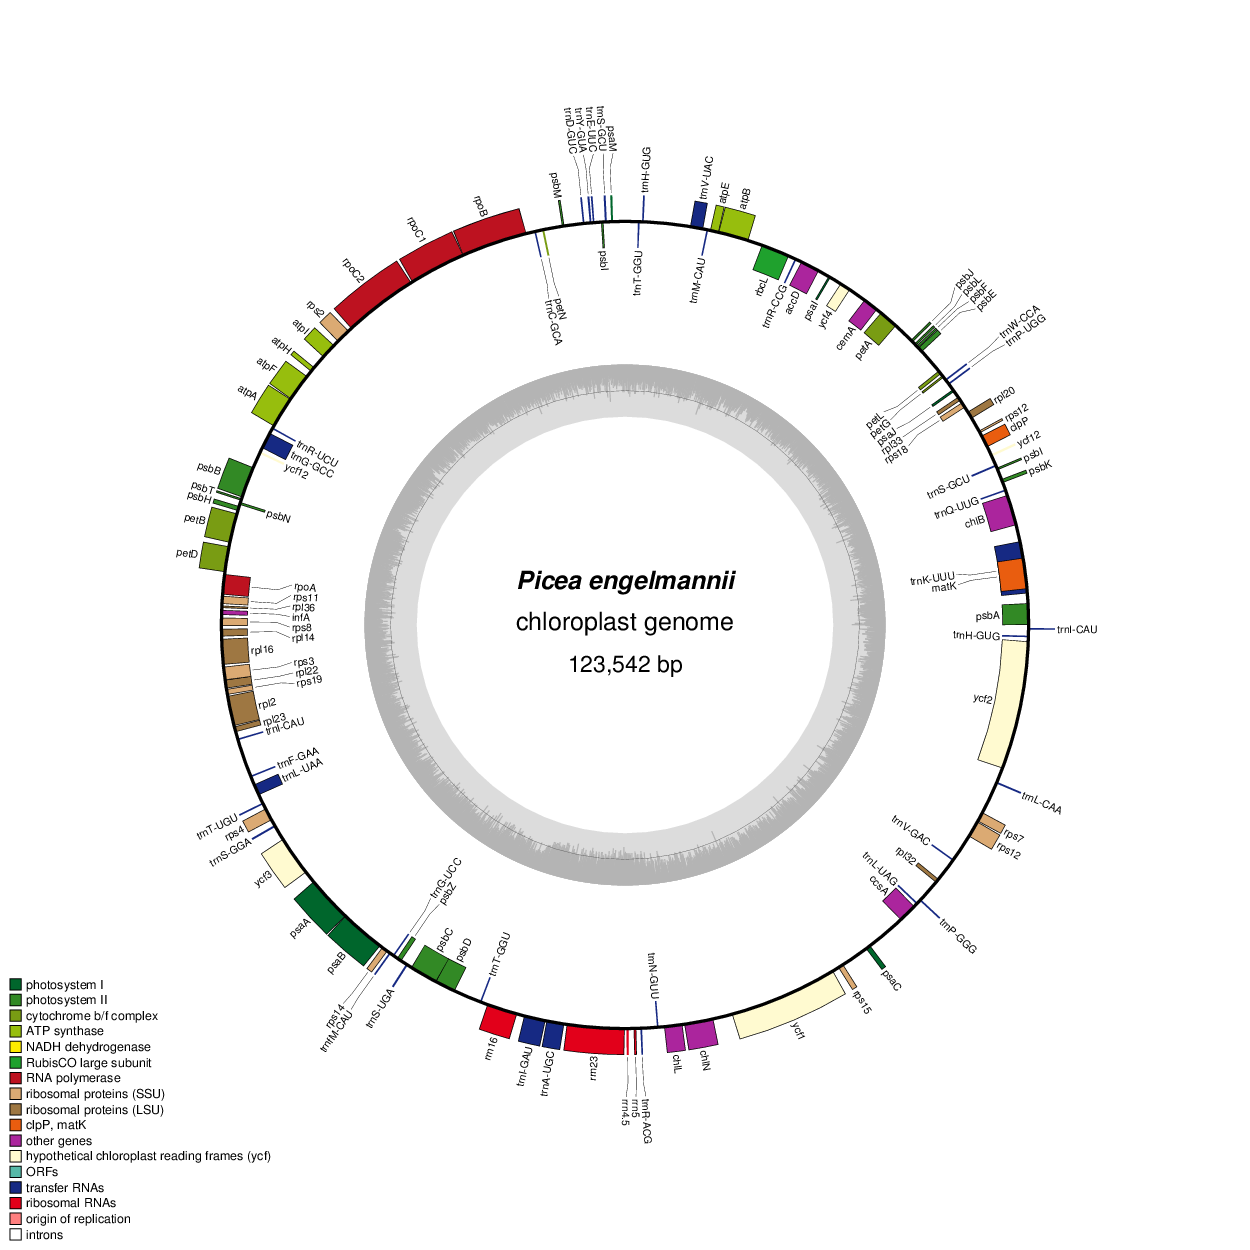
\includegraphics[width=1.0\textwidth]{Se404-851}
\label{fig:ogdraw}
\end{figure}
\end{document}